% Todo Betere titel vinden
\chapter{Onderzoek: Externe bibliotheken gebruiken en het gevaar hiervan}\label{ch:externeGevaren}
Dit hoofdstuk beschrijft het onderzoek wat gedaan is om meer inzicht te krijgen in het doen van een SOUP-analyse. Als eerst wordt de onderzoeksvraag ontleed in te beantwoorden deelvragen. Daarna zal er wordt iedere deelvraag beantwoord om vervolgens tot een conclusie te komen welke de onderzoeksvraag beantwoord.


\section{Onderzoeksvragen} \label{sec:SOUPOnderzoeksvragen}
De onderzoeksvraag die als startpunt van dit onderzoek geld is:"Hoe kunnen we externe bibliotheken op een veilige manier gebruiken?" of "Hoe kan SOUP op een effectieve manier worden geanalyseerd en hoe maakt dit software veiliger?". Uit deze hoofdvraag kunnen de volgende deelvragen worden ontleed:
\begin{itemize}
    \item Wat is veilige software?
    \item Wat is SOUP?
    \item Wat dragen externe bibliotheken en dus ook potentieel SOUP bij aan de ontwikkeling van software?
    \item Wat zijn de gevaren van het gebruik van SOUP?
    \item Wordt er ergens bijgehouden of een dependency/component) een kwetsbaaheid bevat?
    \item Wat relateert SOUP tot software veiligheid binnen EagleScience?
\end{itemize}

%Goed verhaal over supplychain Attacks : https://learning.oreilly.com/library/view/alice-and-bob/9781119687351/c01.xhtml#head-2-27


\section{Wat is veilige software?}
Veilige software is een applicatie dat ontworpen is met onder andere de CIA Triad(confidentiality(vertrouwelijkheid), integrity(integriteit), and availability(beschikbaarheid)) figuure:~\ref{fig:CIA}) in het oog. Dit wil zeggen dat de informatie binnen een applicatie aan de volgende zaken moet voldoen.
\begin{figure}[H]
    \centering
    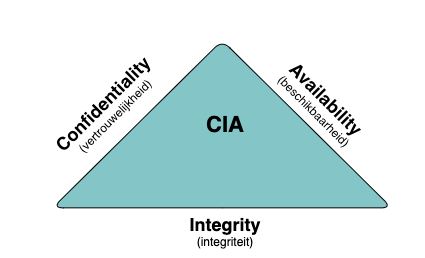
\includegraphics[width=6cm]{gfx/CIA}
    \caption{C.I.A Triad}
    \label{fig:CIA}
\end{figure}

\begin{itemize}
    \item \textbf{vertrouwelijk}: Alleen degene die het recht hebben om de informatie in te zien kunnen deze informatie inzien.
    \item \textbf{integer}: De informatie welke opgeslagen en gebruikt wordt is daadwerkelijk de juiste informatie
    \item \textbf{beschikbaar}: De informatie is beschikbaar op het moment dat het nodig is.
\end{itemize}
Deze drie kernwoorden zorgen ervoor dat als er goed over nagedacht is tijdens de ontwerpfase een goed beeld kan ontstaan hoe een goede applicatie ontwikkeld dient te worden.

Daarnaast zijn er nog een aantal lagen van veiligheid die in een applicatie gebouwd kunnen worden.
Een binnen EagleScience toegepast voorbeeld zou zijn(zie figuur~\ref{fig:veiligheidslagen}):

\begin{figure}[H]
    \centering
    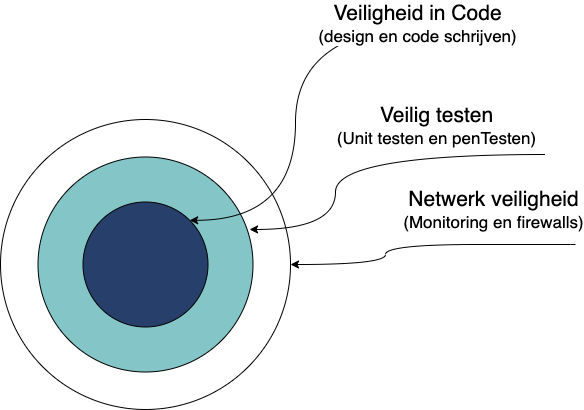
\includegraphics[width=6cm]{gfx/veiligheids lagen}
    \caption{Veiligheids lagen}
    \label{fig:veiligheidslagen}
\end{figure}

\begin{itemize}
    \item \textbf{Tijdens de ontwikkeling van software} is het van belang om de juiste security requirements op te nemen in de requirements documentatie, En dat deze middels, veilige ontwerp concepten worden toegepast,'secure coding tactics', (penetration)testing door verschillende personen en tools worden nageleefd.
    \item \textbf{Tijdens de levensduur van de applicatie} dient de monitoring, op netwerkverkeer en events goed in de gaten gehouden worden dan al niet middels tools en triggers.
    \item \textbf{fysieke beveiliging} De laatste vorm van beveiging zijn daadwerkelijk sleutels op fysieke sloten van de server ruimte en de beslissingen wie deze sleutels heeft.
\end{itemize}
Door deze drie lagen te hanteren heeft EagleScience het ontwikkelen van veilige software in de hand. Daarnaast wordt de OWASP TOP-10 als guideline gebruikt om te zien op welke zaken er gelet dient te worden. De OWASP Top-10 wordt iedere 5 jaar uitgegeven en geeft een beeld van de meest vookomende veiligheidslekken. in 2021 staat op plaats 6 een item over kwetsbare en oude componenten.


\section{Externe Componenten}\label{sec:software-of-unkown-provenance}
Binnen EagleScience bestaat er geen applicatie dit op enig manier gebruik maakt van extern ontwikkelde componenten. Componenten in deze zin zijn ook de runtime-omgevingen die aangemaakt worden door Docker, de kubernetes service waar we gebruik van maken, Zelfs de cloud service is niet van onze maar wordt aangeboden door Microsoft in de vorm van Azure. En zelfs in de componenten binnen de applicaties maakt EagleScience gebruik van externe bronnen(zie Hoofdstuk~\ref{ch:onderzoek:-architectuur-binnen-eaglescience}). Dit Laatste onderdeel is onderwerp van dit onderzoek waarbij er verder ingegaan wordt in het gebruik van externe bibliotheken, ook wel SOUP genoemd, alsook het gevaar hiervan.

\subsection{Wat is Software of Unkown Provenance(SOUP)?}\label{subsec:wat-is-soup?2}
De term SOUP komt oorspronkelijk de wereld van de ontwikkeling van medische software en staat voor "Software Of Unkown Provenance".
SOUP wordt gezien als een software component dat al ontwikkeld is en beschikbaar is gesteld voor gebruik door een instantie anders dan de gebruiker zonder dat de bewijzen zijn over de manier van ontwikkeling als de kwaliteit van de software.
Hierdoor is het dus niet duidelijk welk process er is gevolgt tijdens het ontwikkelen en daarmee dus ook de (medische)veiligheid niet is aan te tonen.
De term wordt nu steeds vaker gebruikt in de algemene software ontwikkel kringen om aan te geven dat er van een betreffent software component(framework, bibliotheek, etc.) niet bekend is hoe het ontwikkeld, getest is.
Hierdoor is er dus geen zekerheid dat het component kwetsbaarheden kan bevatten.
Kwetsbaarheden in deze zin zijn dan voornamelijk lekken of veranderingen van functionaliteiten binnen een software.

\sebsection{Wat dragen externe bibliotheken en dus ook potentieel SOUP bij aan de ontwikkeling van software??}
Als het over het algemeen niet bekend is hoe een bibliotheek of framework gemaakt wordt, waarom zouden we dan het risico lopen om deze dan toch te gebruiken? Het antwoord is vrij simpel: Tijd en Geld. Een applicatie ontwikkelen kost nou eenmaal tijd en dus geld. Op het moment dat er software hergebruikt kan worden levert dit potentieel een tijdswinst op.

Als we een framework genaamd Angular CLI als voorbeeld nemen, neemt dit veel van de taken en mechanismen over in het ontwikkelen van een frontend. Het is wordt dan makkelijker om steeds de zelfde zaken in een frontend voor elkaar te krijgen. Daarnaast zeker in het geval van Angular wat veel gebruikt worden en daarmee een grote community heeft is de supprt vaak snel en doeltreffend. Een ander meekomend voordeel is dat als er 'defacto' frameworks gebruikt worden het intwerken van nieuwe ontwikkelaars minder tijd in beslag neemt omdat de kans dat er elders met in dit geval Angular gewerkt wordt groot is.

Met het overnemen van herhalende taken, makkelijkere opleiden van personeel in acht genomen kan er dus een kortere tim-to-market gehaald worden. ondanks het feit dat er potentieel kwetsbaarheden in de applicatie worden genomen.

\subsection{Hoe relateert SOUP zich met het ontwikkelen van veilige software?}\label{subsec:hoe-relateert-soup-zich-met-het-ontwikkelen-van-veilige-software?}
%Bron: Contrast Security >> https://cdn2.hubspot.net/hub/203759/file-1100864196-pdf/docs/Contrast_-_Insecure_Libraries_2014.pdf

%STATE OF SOFTWARE SECURITY
%Open Source Edition https://www.veracode.com/sites/default/files/pdf/resources/reports/state-of-software-security-open-source-edition-veracode-report.pdf
Uit onderzoek van veraCode blijkt dat 96\% van software ontwikkelende bedrijven gebuik maakt van opensource software. En dat 70,5\% van de applicaties die daadwerkelijk voor het eerst gescanned zijn kwetsbaarheden bevat middels bibliotheken van buitenaf. Het probleem ligt hier niet zozeer in de kwetsbaarheden van een bibliotheek. Maat meer in de kwetsbaarheden in bibliotheken die door de eerste bibliotheken wordt gebruikt. de zogenaamde translative bibliotheken.


Om deze vraag te kunnen beantwoorden moeten we eigenlijk twee zaken onderzoeken als eerste Waarom gebruiken we soup en ten tweede wat wordt er gedaan om veilige software te ontwikkelen.

De voornaamste redenen om bibliotheken te gebruiken is het verminderen van het herhaaldelijk schrijven van code om basis functionaliteiten in een applicatie te krijgen. En Daarmee wordt de ontwikkeltijd verminderd. Het gebruik van bibliotheken is tegenwoordig niet meer weg te denken uit de ontwikkelstrategie van een bedrijf. Deels omdat er een standaard is waarmee gewerkt wordt, wat op zijn beurt het aannemen en opleiden van personeel vergemakkelijkt. Daarnaast hebben veel gebruikte bibliotheken een 'community' waar vragen gesteld kunnen worden om zo moeilijkheden te verminderen. Een nadeel zoals hierboven is beschreven is dat het niet altijd duidelijk is hoe veilig een bibliotheek is.


%Bron: "https://johner-institute.com/articles/software-iec-62304/soup-and-ots/"


\section{Hoe kan het gebruik van SOUP gevaarlijk zijn?}\label{sec:hoe-kan-het-gebruik-van-soup-gevaarlijk-zijn?}
Zoals inmiddels duidelijk bestaat een software component uit een mix van eigen geschreven source code en source code die geschreven staat in bibliotheken dan al niet van derden, zogenoemde depenencies. Deze regel geldt dus niet alleen voor de applicaties die door EagleScience is geschreven, maar dan ook voor de dependencies die gebruikt worden voor de geimporteerde dependency. Dit gaat resursief door totdat we bij dependencies aankomen die zelf geen dependencies gebruiken om hun taak te voltooien. Dit wordt ook wel een dependency tree genoemd. figuur ~\ref{fig:dependency-tree} geeft een verkapte versie weer waarin geillusteerd wordt hoe snel het aantal dependencies optelt.
\begin{figure}[H]
    \myfloatalign
    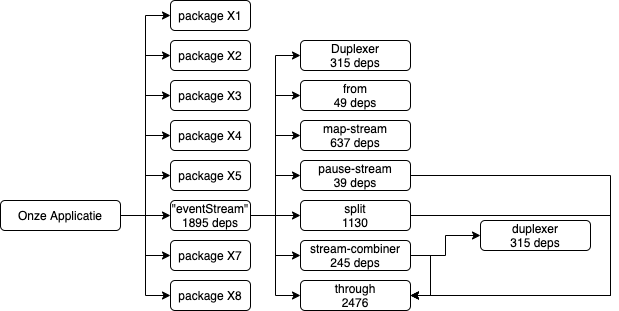
\includegraphics[width=12cm]{gfx/dependency-tree}
    \caption{Dependency tree}\label{fig:dependency-tree}
\end{figure}


\section{Wordt er ergens bijgehouden of een (dependency/component) een kwetsbaaheid bevat?}\label{sec:item-wordt-er-ergens-bijgehouden-of-een-dependency/component)-een-kwetsbaaheid-bevat?}
Naast de OWASP zijn er nog een aantal instanties die zich bezighouden met het veilighouden van software. Vaak is dit het verzamelen van kwetsbaarheden en deze vind en kenbaar maken aan het publiek. Twee instituten die samenwerken zijn MITRE en Information TechnologyLab van het NIST\footnote{National Institute of Standards and Technology: Instituur onder amerikaanse regering die verschillende onderzoeken doen op het het gebied van technologie}TL van

\subsection{CVE Databases, MITRE, NIST, NVD}\label{subsec:mitre-nist-nvd}
CVE staat voor Common Vulenerabilities en Exposures wat een database waarin kwetsbaarheden staan die gevonden zijn in de verschillende systemen.
Deze Database wordt voornamelijk bijgehouden door het bedrijf MITRE dat met subsidie van de US Division of Homeland Security werkt aan het kenbaar maken van lekken in software\footnote{Software wordt hier gezien in de ruimste zin van het woord hierbij hoort: Operating systems, open en closed source software. maar ook frameworks en bibliotheken.}.
De CVE's die in deze database staan worden vervolgens geannalyseerd door het NIST(National Institute os Standards and Technology) en voorzien van een CVSS\footnote{Common Vulnerability Score System is een gestandardiseerde manier om een score aan een kwetsbaarheid toe te kennen waarop in een enkel oog opslag te zien is hoe rieel een risico is.} score en geplaats in de NVD-database.
Zowel de database van MITRE (https://cve.mitre.org) als NIST (https://nvd.nist.gov) zijn publiekelijk toegankelijk.

\subsection{OWASP}\label{subsec:owasp}
Naast het bijhouden van CVE's in database is het creëren van awareness net zo belangrijk.
Een instantie die zich bezig houd hier mee is OWASP(Open Web Application Security Project) die awareness creëert door ideree 5 jaar een Top-10 uit te brengen met daarin de meest voorkomende en dreigende kwetsbaarheden die ze gevonden hebben in een dataset wat opgebouwd is uit inzendingen van 500+ onderzoekers van 40+ bedrijven die samen meer dan 100.000 API's en web applicaties hebben onderzocht.
In de top 10 die hieronder samengevat weer wordt gegeven wordt er een score meegegeven over hoe makkelijk een lek is te ontdekken en welk mate van risico de kwetsbaarheid heeft.

\begin{figure}[H]
    \myfloatalign
    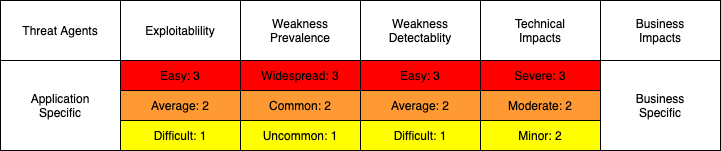
\includegraphics[width=12cm]{gfx/risk tabel}
    \caption{Inschaling van risico's door OWASP}
    \label{fig:risico inschaling}
\end{figure}


%Bronnen:
%https://www.imperva.com/learn/application-security/cve-cvss-vulnerability/
%http://owasp.org


\section{Invloed van SOUP op veiligheid van software}\label{sec:invloed-van-soup-op-veiligheid-van-software}
In de OWASP top-10 staat op plaats 9 "Using components with known vulnerabilities" wat aangeeft dat het op het moment van schrijven aandacht nodig heeft.
Eén van de redenen dat dit probleem in de top 10 staat is omdat het gebruik van bibliotheken bijna niet te vermijden is in de ontwikkeling van applicaties wat vooral te danken is aan het steeds sneller moet leveren van een product.
Ontwikkelaars zijn nooit volledig op de hoogte van de werking laat staan wie de onwikkelaar is van een externe bibliotheek.
Een goed voorbeeld hiervan is de "event-stream vulnerability" waarbij de bibliotheek voorzien werd van crypto-coin-stealing malware.
Dit kon gebeuren omdat de bibliotheek niet meer actief werd onderhouden en een persoon zich aanmelde om de ontwikkeling over te nemen.
Vervolgens werd een dependency omgezet van versie en functionaliteit waardoor er toegang werd, verleent om crypto coins te stelen.
Event-stream is een bibliotheek dat veel gebruikt werd als dependency voor applicaties de stream-functionaliteiten van nodejs gebruikten daardoor heeft het de potentie gehad om veel schade aan te richten.
Het is niet geheel duidelijk hoeveel schade er is gelden echter laat dit voorbeeld duidelijk zien wat het probleem is en hoe snel je kan verdwalen in dependency tree's.
Een oplossing is om regelmatig te scannen naar verdachte bibliotheken in de dependency tree.
En er vervolgens actief mee om te gaan door bibliotheken up-to-date te houden.
%Bron: https://www.theregister.com/2018/11/26/npm_repo_bitcoin_stealer/


\section{Dependency trees?}\label{sec:dependency-trees?}



[NOTE Volgende komt uit SOUP ANALYSE hoofdstuk]

\begin{itemize}
    \item https://jeremylong.github.io/DependencyCheck/
\end{itemize}

Voordat we verder kijken naar mogelijkheden om kwetsbaarheden in een externe bibliotheek te onderzoeken en te verhelpen moeten we eerst kijken naar een aantal kernbegrippen om te begrijpen waar het om gaat.

Dit onderzoek heeft daarom ook twee hoofdvragen die ieders weer een aantal deelvragen opwerpen.
Als eeste is de vraag "Welke kwetsbaarheden bestaan er hoe is het gebruik van externe bibliotheken hier aan gecorreleerd?
De deelvragen die hier uit voorkomen luiden:
\begin{itemize}
    \item Wat zijn applicatie veiligheidsrisico's?
    \item Welke komen het meest voor?
    \item
\end{itemize}


\section{Wat zijn applicatie veiligheidsrisico's}\label{sec:wat-zijn-applicatie-veiligheids-risico's}
Veiligheids risico's binnen applicaties zijn een som van kwetsbaarheden die zich bedoeld of onbedoeld in de applicatie bevinden, de vindbaarheid en de "schade" die er mee aangericht kunnen worden.
De termen van de som worden hieronder verder uitgediept als ook een top-10 uitgeven door de OWASP van de meest voorkomende kwetbaarheden.

Een aanvaller kan op meerdere manier in een applicatie komen(figuur X).
Vaak gebeurt dit door een kwetsbaarheid van een applicatie te zoeken en deze te exploiteren.
Als er vervolgens geen maatregeling genomen zijn om de aanvaller te weerhouden kunnen er zaken als data in een database, assets van het bedrijf of zelfs functionaliteit aangetast worden.
Wat op zijn beurt weer voor een impact in de bedrijfsvoering kan veroorzaken.
Hoe aanvallers een applicatie kunnen aanvallen is applicatie specifiek
De impact op de bedrijfsvoering is ook specifiek
\begin{figure}[H]
    \myfloatalign
    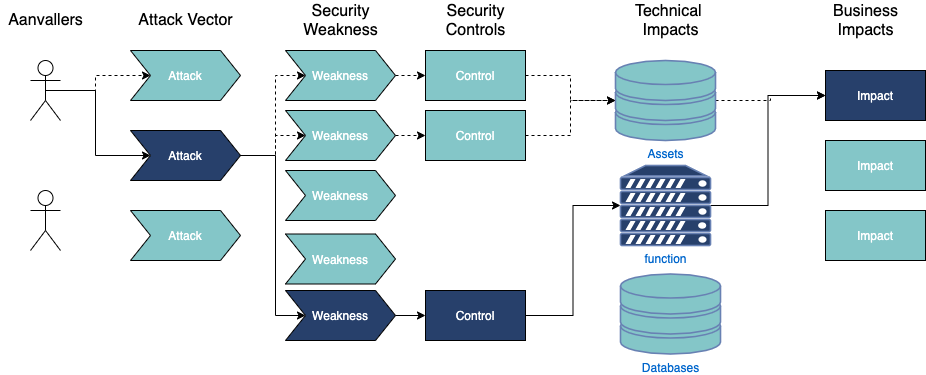
\includegraphics[width=15cm]{gfx/application security routes}
    \caption{Aanvalllen, en hun gevolg}
    \label{fig:Application Security Routes}
\end{figure}

Veiligheids risico's kunnen in categoriën worden geplaatst middels een gradatie systeem die in figuur x te ze zien is.
De OWASP-Top10 die verder in de tekst te vinden is maakt gebruik van dit gradatie systeem om risico's in te schalen.
OWASP is een instantie die zich bezighouden met het verbeteren van de veiligheid van applicaties.
Het doet dit door onder andere training en erkenning te geven aan kwetsbaarheden.
Zo wordt er eens in de 5 jaar een top-10 samengesteld met de op dat moment meest voorkomende kwetsbaarheden.
\footnote{Helaas is de laatste versie die aan het einde van 2021 uit moet komen nog niet beschikbaar op het moment van schrijven}
De OWASP-Top10 wordt samengesteld uit data van meer dan 100.000 productie applicaties en APIs wat door meer dan 500 mensen is getest door 40 verschillende bedrijven.
De top 10 is een aggegratie van deze data in de meest voorkomende issues met inachtneming van exploitabity, detectability en impact.


%\begin{figure}[H]
%  \myfloatalign
%  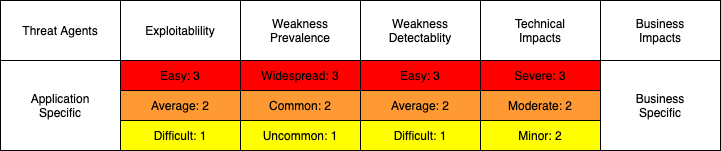
\includegraphics[width=12cm]{gfx/risk tabel}
%  \caption{Inschaling van risico's}
%  \label{fig:risico inschaling}
%\end{figure}

%threat agents = aanvallende entiteit
%exploitabity = exploiteetbaatheid
%weakness prevalance = vookomendheid van de zwakte in een applicatie
%weakness detectability = hoe goed is de zwakte in een applicatie te detecteren
%technical impact = technische impact op de applicaties
%business impacts = (zakelijke impact) impact op de bedrijfsvoering





\

Binnen Eaglescience wordt er heel goed gekeken naar de manier waarop er veilige software ontwikkeld wordt.
Zaken die in de OWASP top-10 staan wordt serieus mee omgegaan en actief tegen gehandeld. zo wordt er ook gegekeken naar het gebruik van bibliotheken van derden.

Op plaats A09:2017 is te vinden dat er kwetsbaarheden middels bibliotheken van derden binnen kunnen komen. Dit is iets wat deels buiten het bereik van Eaglescience ligt. Om ons hier tegen te beschermen is het wenselijk om periodiek en geautomatiseerd een analyse naar kwetbaarheden tedoen.

De bibliotheken die gebruikt worden van derden wordt ook wel Software of unkown pedigree genoemd of kortweg SOUP. Dit houdt in dat een bibliotheek wordt ontwikkeld middels een proces of methode wat niet bekend is bij de eindgebruiker. Ook zijn vaak de details niet bekend van de bibliotheek omdat deze niet of nauwelijks wordt gereviewed door de eindgebruiker. Om deze reden is het dus onbekend of er kwetsbaarheden zitten in betreffende bibliotheken.
De definitie van SOUP blijft niet alleen bij de bibliotheken en frameworks vanuit het open-source gebied. Veelal is ook niet bekend hoe closed-source (Proprietary software) wordt geschreven, echter door reputatie van bedrijven die deze software schrijven wordt veelal , onterecht\footnote{zie: https://www.nu.nl/tech/6097701/waarom-de-hack-bij-solarwinds-ministeries-en-grote-bedrijven-treft.html } aangenomen dat deze geen lekken bevatten.


\section{CVE}
in de appliction security wordt er gesproken van een CVE(Common Vulnerability en Exposures) als een kewtsbaarheid bekend is deze wordt in een database geplaatst zodat \'e\'en ieder die geintreseerd is hier kan vinden welke software(os, applicatie, framework, bibliotheek) mogelijk niet veilig is. Deze Database wordt in stand en bijgehouden door een aantal instanties waarbij de belangrijksten zijn:
\begin{itemize}
    \item \textbf{NIST-CSRC} Computer Security Research Center van het National Institute of Standards and Technology) is een centrum dat onderzoek doet namens de Amerikaanse regering naar veiligheden in software. De database die het NIST-CSRC bijhoud heet het NVD(National Vulnerability Database) waarin CVE's worden bijgehouden.
    \item \textbf{CVE-Mitre} is een community driven effort wat CVE's logt in een lijst die vervolgens de NVD voedt met hun gevondendata.
    \item \textbf{cvedetails.com/}
    \item \textbf{vuldb.com/}
    \item \textbf{https://www.exploit-db.com/}
\end{itemize}


\section{}

https://www.security.nl/posting/666663/Van+CVE+tot+CVSS\%3A+wegwijs+in+het+woud+van+kwetsbaarheden










